\begin{figure}
    \centering
\begin{knitrout}
\definecolor{shadecolor}{rgb}{0.969, 0.969, 0.969}\color{fgcolor}
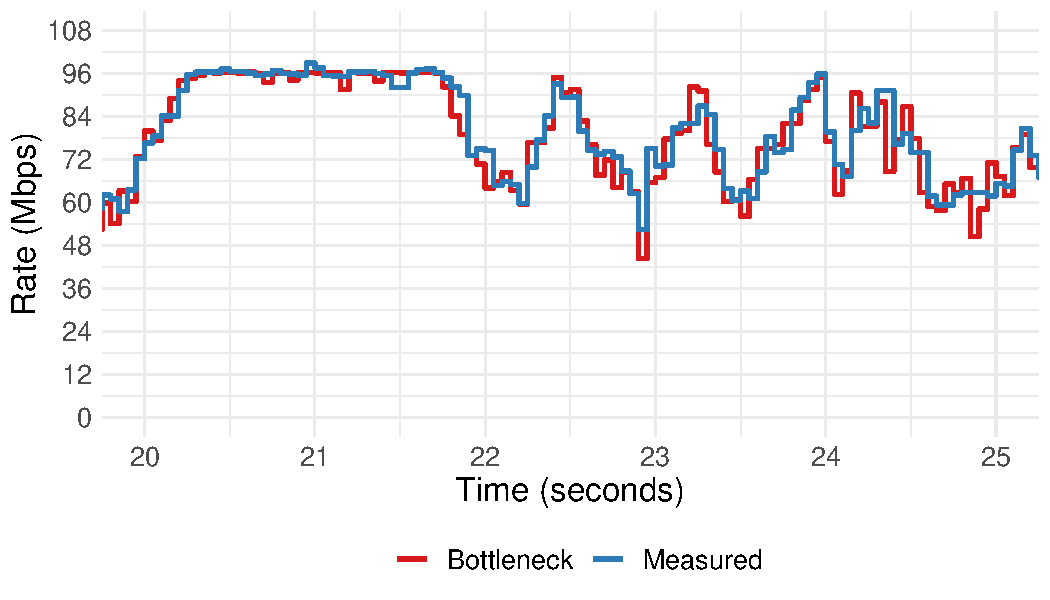
\includegraphics[width=\maxwidth]{figure/micro:time-thru-1} 

\end{knitrout}

    \caption{The distribution of the error of \name's measurements across a range of network conditions. The vast majority of \name's estimates are within a small fraction of the actual value. The dashed lines show the 10th, 50th, and 90th percentile, and the edges of the plot contain the 1st and 99th percentiles.}
    \label{fig:micro:time-thru}
\end{figure}
